\documentclass[11pt,a4paper]{article}
\usepackage[margin=2.3cm]{geometry}
\usepackage{xeCJK}
\setCJKmainfont{NotoSansCJKsc-Regular.otf}[Path=fonts/,BoldFont=NotoSansCJKsc-Bold.otf]
\setCJKsansfont{NotoSansCJKsc-Regular.otf}[Path=fonts/,BoldFont=NotoSansCJKsc-Bold.otf]
\usepackage{amsmath,amssymb,amsthm}
\usepackage{graphicx}
\usepackage{booktabs}
\usepackage{xcolor}
\usepackage{enumitem}
\usepackage{caption}
\usepackage[colorlinks=true,linkcolor=blue,urlcolor=blue,citecolor=blue]{hyperref}
\usepackage{tcolorbox}
\tcbuselibrary{skins,breakable}

\definecolor{deepblue}{HTML}{2B6CB0}
\definecolor{deepred}{HTML}{C53030}
\definecolor{deepgreen}{HTML}{2F855A}
\definecolor{warn}{HTML}{DD6B20}

\setlength{\parindent}{2em}
\setlength{\parskip}{0.35em}
\linespread{1.28}
\captionsetup{font=small,labelfont=bf,justification=centering}

\newtcolorbox{keybox}[1][]{enhanced,breakable,colback=blue!3,colframe=deepblue,
  boxrule=0.6pt,arc=2pt,left=6pt,right=6pt,top=5pt,bottom=5pt,
  fonttitle=\bfseries,title=#1}
\newtcolorbox{warnbox}[1][]{enhanced,breakable,colback=orange!4,colframe=warn,
  boxrule=0.6pt,arc=2pt,left=6pt,right=6pt,top=5pt,bottom=5pt,
  fonttitle=\bfseries,title=#1}

\title{\bfseries 一堂关于纳维–斯托克斯方程的公开课\\[4pt]
\large 为什么二维能证完、三维却不能；以及 2026 年那场“AI 证明了千禧问题”到底证明了什么}
\author{配套材料：论文 \texttt{paper/ns-forced-vs-unforced.pdf}、代码 \texttt{notes/make\_figs.py}}
\date{2026 年 11 月}

\renewcommand{\abstractname}{导读}
\renewcommand{\contentsname}{目录}
\renewcommand{\figurename}{图}
\renewcommand{\tablename}{表}
\renewcommand{\appendixname}{附录}
\renewcommand{\refname}{参考文献}

\setcounter{topnumber}{3}
\setcounter{bottomnumber}{2}
\setcounter{totalnumber}{4}
\renewcommand{\topfraction}{0.85}
\renewcommand{\bottomfraction}{0.65}
\renewcommand{\textfraction}{0.1}
\renewcommand{\floatpagefraction}{0.75}

\begin{document}
\maketitle

\begin{abstract}
\noindent
这份讲义面向“数学不错、但不是这个方向”的读者。目标只有三个：
（一）用图示讲清楚纳维–斯托克斯方程在问什么，什么叫“解爆破”；
（二）讲清楚为什么二维情形已经被人类完全解决，而三维卡了九十多年——差别只有一项；
（三）把 2026 年 9--10 月那场“AI 证明了千禧问题”的新闻拆开：它到底证了什么、
没有证什么、为什么“带外力”和“不带外力”是两个不同的问题。
所有图都是本仓库重新画的；其中二维涡量的四张快照和 $L^p$ 范数曲线来自
一次真实的数值模拟（谱方法，$192^2$ 网格），不是示意图。
\end{abstract}

\tableofcontents

\section{先给结论：三句话}

\begin{keybox}[本文的三句话]
\begin{enumerate}[leftmargin=1.6em]
\item \textbf{二维已经证完。} 二维不可压缩纳维–斯托克斯方程，对任意光滑初值都存在
      永远光滑的解——这是定理，不是猜想。
\item \textbf{三维仍然开放。} 三维情形正是 Clay 数学研究所 2000 年悬赏 100 万美元的
      千禧问题之一：没人能证明解永远光滑，也没人能构造出真正爆破的解。
\item \textbf{2026 年的“AI 证明”证的是“带外力”的版本。} 一旦允许外加的体积力，
      方程就变成了一个\emph{控制问题}：你可以让流体沿着几乎任意预设的路径走
      （本文第 \ref{sec:prescription} 节会给出严格定理）。代价是：这个外力必须在
      爆破时刻按 $(T-t)^{-3/2}$ 的速度发散。去掉外力，问题原封不动。
\end{enumerate}
\end{keybox}

如果你只记住一句话：\emph{“三维纳维–斯托克斯有没有爆破”这个问题，到今天为止，
既没有被证明“有”，也没有被证明“没有”；2026 年的新闻解决的是另一个（更弱的）问题。}

\section{方程在说什么}

\subsection{一句话版本}

纳维–斯托克斯方程就是“牛顿第二定律，用在流体上”：
\[
\underbrace{\partial_t u}_{\text{速度变化}}
+\underbrace{(u\cdot\nabla)u}_{\text{被自己带着走}}
-\underbrace{\nu\Delta u}_{\text{粘性摩擦}}
+\underbrace{\nabla p}_{\text{压力}}
=\underbrace{f}_{\text{外力}},
\qquad
\underbrace{\operatorname{div}u=0}_{\text{不可压缩}}.
\]
其中 $u(x,t)\in\mathbb{R}^3$ 是速度场，$p$ 是压力，$\nu>0$ 是粘性系数
（水约为 $10^{-6}\,\mathrm{m^2/s}$，蜂蜜要大得多），$f$ 是外力（重力、搅拌、电磁力……）。

三个词解释清楚就够了：
\begin{itemize}[leftmargin=1.6em]
\item \textbf{不可压缩}（$\operatorname{div}u=0$）：流体不会被“压扁”，进多少出多少；
\item \textbf{对流项} $(u\cdot\nabla)u$：流体自己带着自己跑，这是方程里唯一的非线性项，
      也是所有麻烦的来源；
\item \textbf{粘性项} $\nu\Delta u$：速度的“凹凸不平”会被抹平，越小的尺度被抹得越快。
\end{itemize}

\subsection{工程师天天在算，数学家却不知道解是否存在}

飞机、天气、血管、管道、赛车，全靠这套方程（或它的简化版）做数值模拟。
工程师用计算机算得很开心，是因为数值格式会悄悄加入“数值粘性”，把麻烦抹掉；
而数学家问的是：\emph{在精确的意义下，这个方程从光滑初值出发，会不会在有限时间内
把解“弄炸”？}

“弄炸”有精确含义：速度本身也许还有界，但它的梯度 $\nabla u$ 会在一瞬间变得无穷大，
之后方程就不再有意义。图~\ref{fig:blowup} 画的正是这件事（示意图）。

\begin{figure}[htbp]
\centering
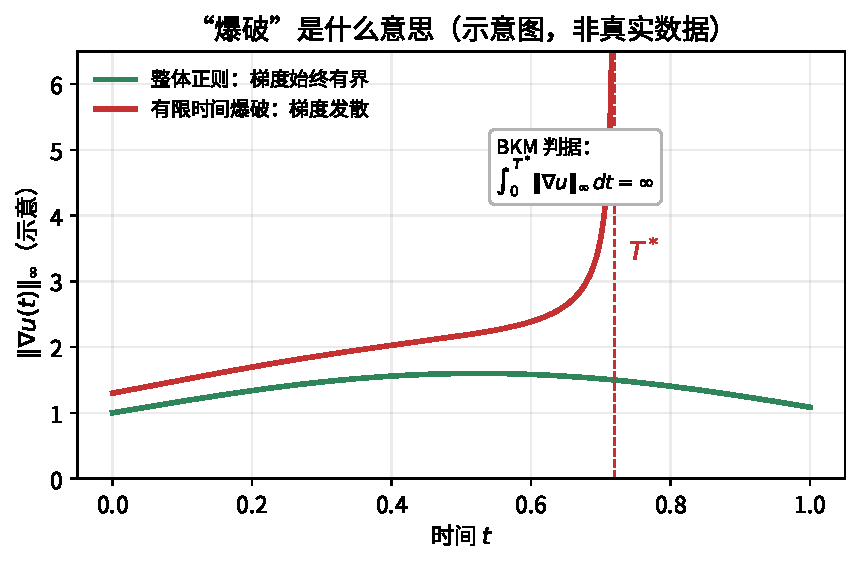
\includegraphics[width=0.72\linewidth]{figs/fig13_blowup.pdf}
\caption{“爆破”是什么意思。绿色：整体正则，梯度始终有界；红色：有限时间爆破，
梯度在 $T^*$ 处发散。这张图是示意，不是真实数据；真实的三维爆破至今没人构造出来。}
\label{fig:blowup}
\end{figure}

顺便说一个漂亮的判据（Beale--Kato--Majda，1984）：
\[
\text{解在 }T^*\text{ 处爆破}
\iff
\int_0^{T^*}\|\nabla u(t)\|_\infty\,dt=\infty .
\]
也就是说，爆破不是“某一刻突然变坏”，而是“梯度在时间上的积分发散”。
这个判据是我们后面理解二维与三维差别的钥匙。

\subsection{千禧问题是怎么问的}

Clay 的官方提法（Fefferman 执笔）大致是二选一：给定 $\mathbb{R}^3$ 上光滑、
紧支撑、无散的初值，粘性 $\nu>0$，且\textbf{没有外力}（$f\equiv0$），
\begin{itemize}[leftmargin=1.6em]
\item[(A)] 存在唯一的整体光滑解；还是
\item[(B)] 存在有限时间就失去光滑性的解？
\end{itemize}
Clay 的官方问题实际上有\textbf{四个变体}：两个无外力（$\mathbb{R}^3$ 与环面），两个带
光滑外力；媒体（以及 \emph{Scientific American} 的报道）把带外力的版本称作选项 (C)。
这次 2026 年的声称瞄准的正是带外力的那两个，无外力的两个原封未动。
\textbf{请注意：(C) 不是 (A)/(B) 的等价改写。} 这是全文最关键的一句话，
第 \ref{sec:prescription} 节会给出严格理由。

\section{二维：为什么能证完}\label{sec:2d}

\subsection{把方程“转 90 度”：涡量}

二维时，把速度场旋转 90 度求散度，可以得到\emph{涡量}
$\omega=\partial_1u_2-\partial_2u_1$（直觉：流体微团自转的快慢）。
对纳维–斯托克斯方程取旋度，压力项消失，得到
\begin{equation}\label{eq:vort2d}
\boxed{\;\partial_t\omega+(u\cdot\nabla)\omega=\nu\Delta\omega\;}
\end{equation}
这是一个\emph{纯输运--扩散}方程：涡量只会被流体“带着走”，再被粘性“抹平”，
\emph{不会}被放大。

关键的一步是乘以 $\omega|\omega|^{p-2}$ 再积分。输运项立刻消失：
\[
\int_{\mathbb{T}^2}(u\cdot\nabla)\omega\;\omega|\omega|^{p-2}\,dx
=\frac1p\int_{\mathbb{T}^2}u\cdot\nabla|\omega|^p\,dx
=-\frac1p\int_{\mathbb{T}^2}(\operatorname{div}u)\,|\omega|^p\,dx=0 .
\]
最后一步用了不可压缩条件 $\operatorname{div}u=0$。这一步是整件事的灵魂：
\emph{“带着走”不改变涡量的整体大小，只有粘性会。}
再配合 Kato 不等式 $\Delta|\omega|^p\ge p|\omega|^{p-2}\omega\Delta\omega$，得到
\[
\frac{d}{dt}\|\omega(t)\|_p\le\|\omega_0\|_p\quad(p\ge2),
\]
即：\textbf{二维涡量的所有 $L^p$ 范数都不随时间增加。}

这既是物理，也是图~\ref{fig:snapshots} 与图~\ref{fig:norms} 的内容——它们来自
一次真实的数值模拟，不是示意。

\begin{figure}[htbp]
\centering
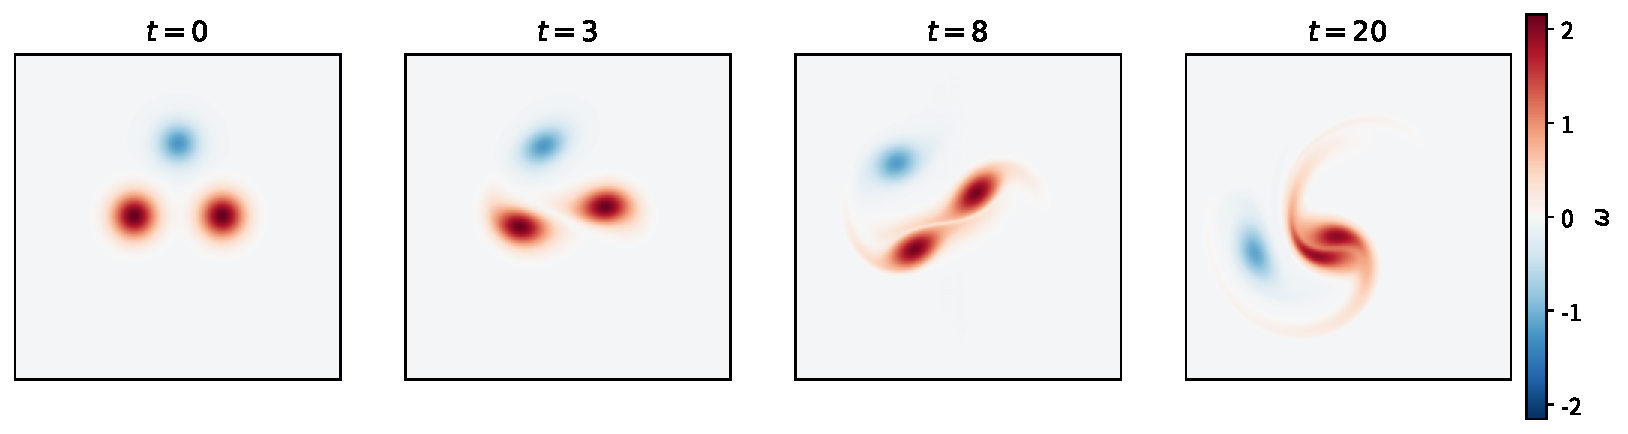
\includegraphics[width=\linewidth]{figs/fig02_2d_snapshots.pdf}
\caption{二维涡量的真实演化（谱方法，$192^2$ 网格，$\nu=2\times10^{-4}$）。
两个同号涡（红）互相绕转、合并，把涡量拉成细丝；上方的反号涡（蓝）被甩开。
注意：涡量被拉成丝，但\emph{峰值并没有变大}——它只是被摊开了。}
\label{fig:snapshots}
\end{figure}

\begin{figure}[htbp]
\centering
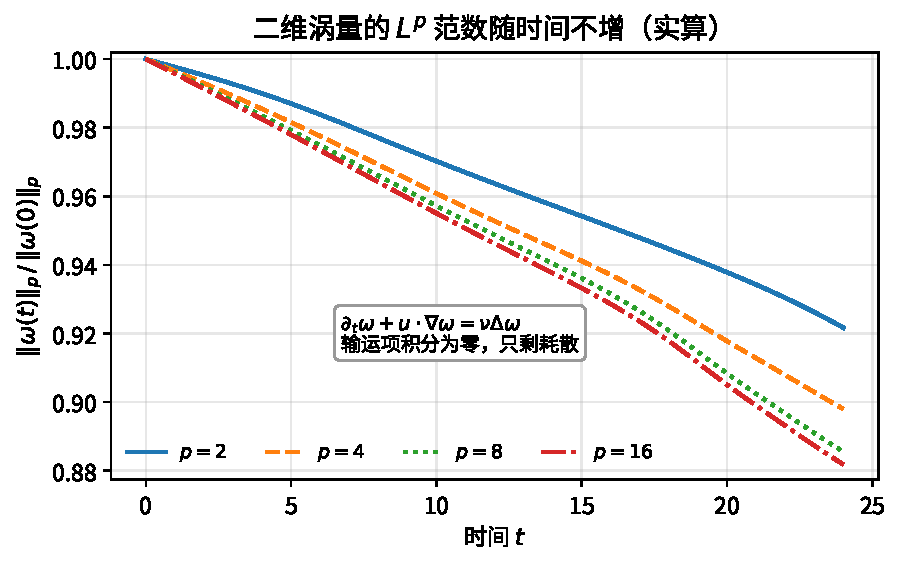
\includegraphics[width=0.78\linewidth]{figs/fig03_2d_norms.pdf}
\caption{同一次模拟中，$\|\omega(t)\|_p/\|\omega(0)\|_p$ 随时间的变化。
四条曲线（$p=2,4,8,16$）全部单调不增，且 $p$ 越大下降越快——这正是上一段的不等式。}
\label{fig:norms}
\end{figure}

\subsection{从涡量到“永不爆破”}

有了 $\|\omega\|_p$ 的一致界，剩下是一条标准的流水线（细节见论文第 5 节）：
\[
\|\omega\|_{L^\infty_tL^p}
\;\Longrightarrow\;
\|\nabla u\|_{L^\infty_tL^p}
\;\Longrightarrow\;
u\in L^\infty ,
\]
\[
u\in L^\infty
\;\Longrightarrow\;
\text{自举（bootstrap）}
\;\Longrightarrow\;
\int_0^T\|\nabla u\|_\infty\,dt<\infty
\;\Longrightarrow\;
\text{不爆破}.
\]
第一步是 Biot--Savart 公式（二维时 $\nabla u$ 是 $\omega$ 的 Riesz 变换）；
最后一步正是 BKM 判据。因为 $T$ 可以任意大，结论就是全局正则性。

\begin{keybox}[二维定理：Ladyzhenskaya 1969]
对任意光滑、无散的初值和任意光滑外力，二维纳维–斯托克斯方程存在唯一的、
对所有 $t>0$ 光滑的解。
\end{keybox}

\subsection{一句话对比}

图~\ref{fig:2d3d} 把二维和三维的涡量方程并排放。差别只有一项：三维多了一个
$(\omega\cdot\nabla)u$。就是这一项，让人类卡了九十年。

\begin{figure}[htbp]
\centering
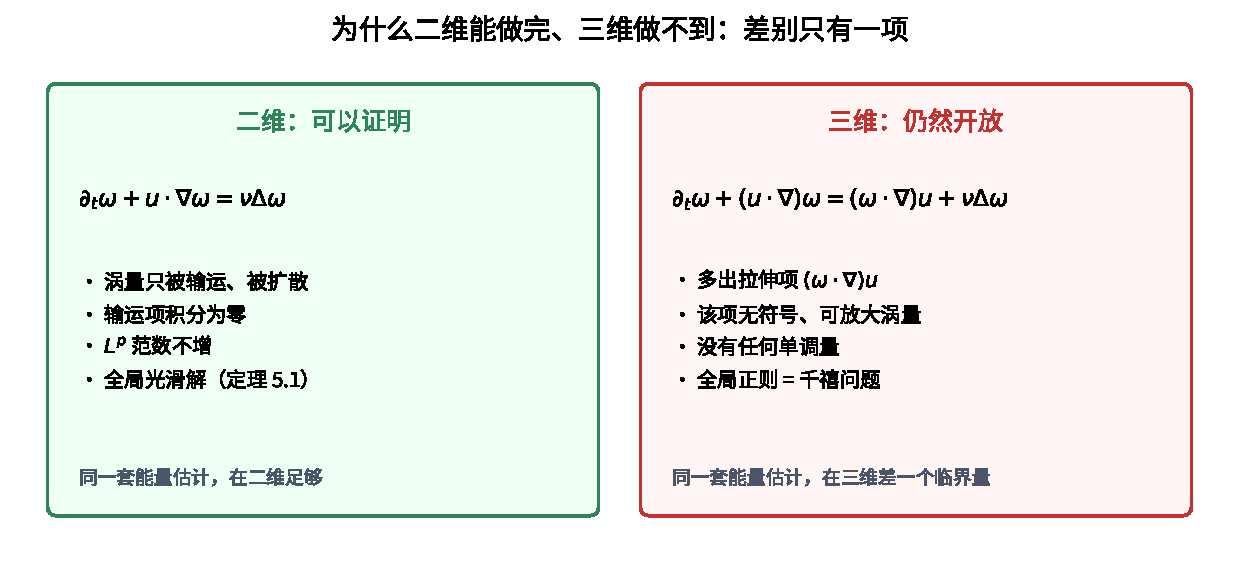
\includegraphics[width=\linewidth]{figs/fig12_2d_vs_3d.pdf}
\caption{二维与三维的唯一差别：三维涡量方程多出拉伸项 $(\omega\cdot\nabla)u$。
它没有符号，可以把涡量放大，于是“范数不增”这一整条论证链断掉。}
\label{fig:2d3d}
\end{figure}

\section{三维：多出来的那一项有多要命}\label{sec:3d}

\subsection{涡管拉伸}

三维的涡量方程是
\begin{equation}\label{eq:vort3d}
\partial_t\omega+(u\cdot\nabla)\omega
=\underbrace{(\omega\cdot\nabla)u}_{\text{拉伸项}}+\nu\Delta\omega .
\end{equation}
拉伸项的物理意义如图~\ref{fig:stretch}：一根涡管被流场拉长，截面变细，
由环量守恒，涡量必须变强。注意这一步\emph{不违反任何守恒律}——它把
“大尺度上的拉伸”转换成“小尺度上的强涡量”，这正是湍流能量级联的几何来源。

\begin{figure}[htbp]
\centering
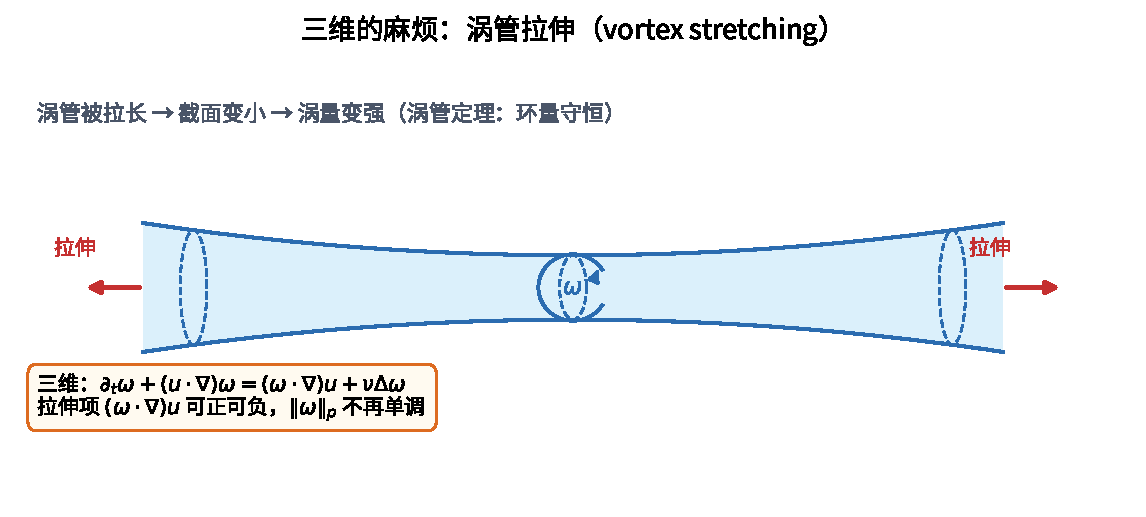
\includegraphics[width=0.94\linewidth]{figs/fig04_stretching.pdf}
\caption{涡管拉伸。管子变长、变细，涡量变强。数学上，这意味着
$\int(\omega\cdot\nabla)u\cdot\omega\,dx$ 没有确定的符号，不能像二维那样直接丢掉。}
\label{fig:stretch}
\end{figure}

\subsection{能量估计为什么“差一点”}

把三维方程乘以 $u$ 积分，对流项照样消失，得到能量恒等式
\[
\frac12\frac{d}{dt}\|u\|_2^2+\nu\|\nabla u\|_2^2=(f,u).
\]
它给出 $\|u\|_{L^\infty_tL^2}$ 和 $\|\nabla u\|_{L^2_tL^2}$ 的界。
问题在于：三维里这两个量\emph{都不足以}控制 $\|\nabla u\|_\infty$。
用 BKM 判据说，我们手上有 $\|\nabla u\|_{L^2_tL^2}$，而需要的却是
$\|\nabla u\|_{L^1_tL^\infty}$——两者之间，正好差一个“尺度”。

这个“差一个尺度”在图~\ref{fig:scaling} 里看得很清楚：把解按
$u_\lambda(x,t)=\lambda u(\lambda x,\lambda^2t)$ 缩放，
\[
\|u_\lambda\|_{L^3}=\|u\|_{L^3}\ (\text{不变}),\qquad
\|\nabla u_\lambda\|_{L^2}\propto\lambda^{1/2},\qquad
\|f_\lambda\|_{L^\infty}\propto\lambda^{3}.
\]
$L^3$ 是“临界的”：它不随尺度变。能量（$L^2$）是“次临界的”：尺度越小，
能量越小，所以能量控制不了小尺度。三维的一切困难，都可以追溯到这个尺度缺口；
二维之所以能做完，是因为二维涡量的 $L^p$ 界恰好补上了这个缺口。

\begin{figure}[htbp]
\centering
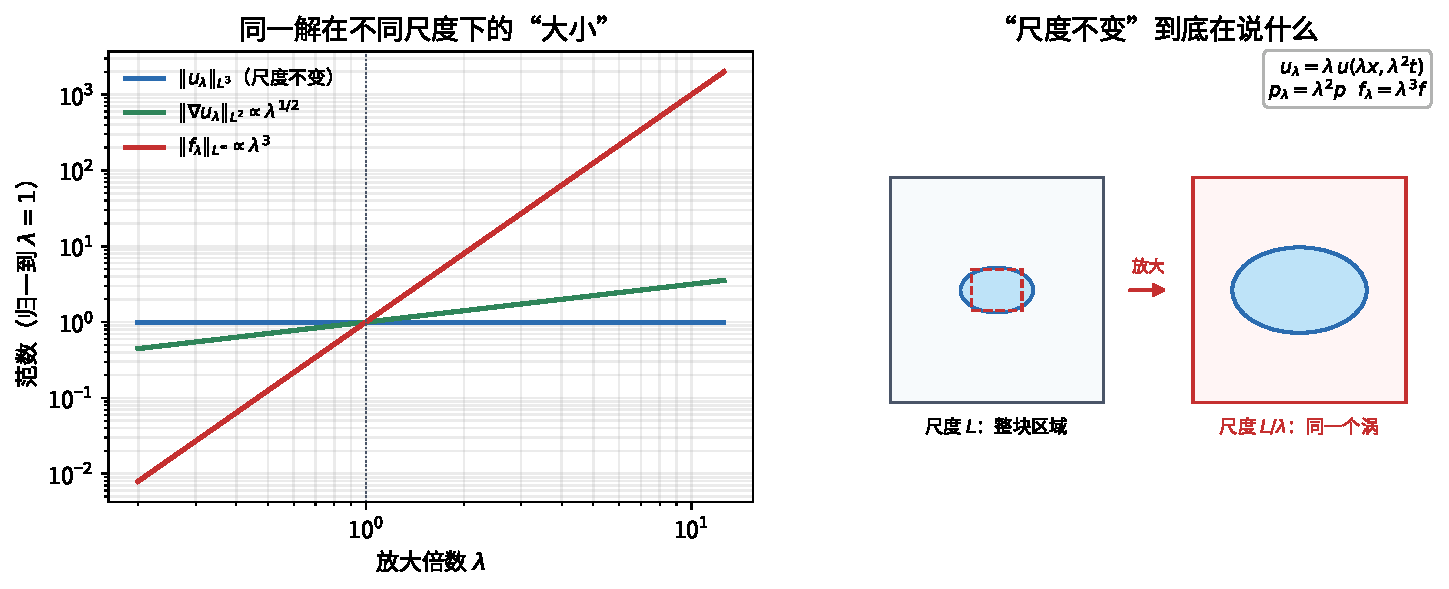
\includegraphics[width=\linewidth]{figs/fig01_scaling.pdf}
\caption{左：同一解在不同尺度下的范数（对数坐标）。$L^3$ 范数是一条水平线（尺度不变），
能量梯度按 $\lambda^{1/2}$ 增长，外力按 $\lambda^3$ 增长。右：缩放到底在做什么——
把同一个涡放大 $\lambda$ 倍看。}
\label{fig:scaling}
\end{figure}

\section{人类已经知道什么（以及不知道什么）}\label{sec:known}

图~\ref{fig:timeline} 是一张时间线。这里把四个必须知道的结果说清楚。

\begin{figure}[htbp]
\centering
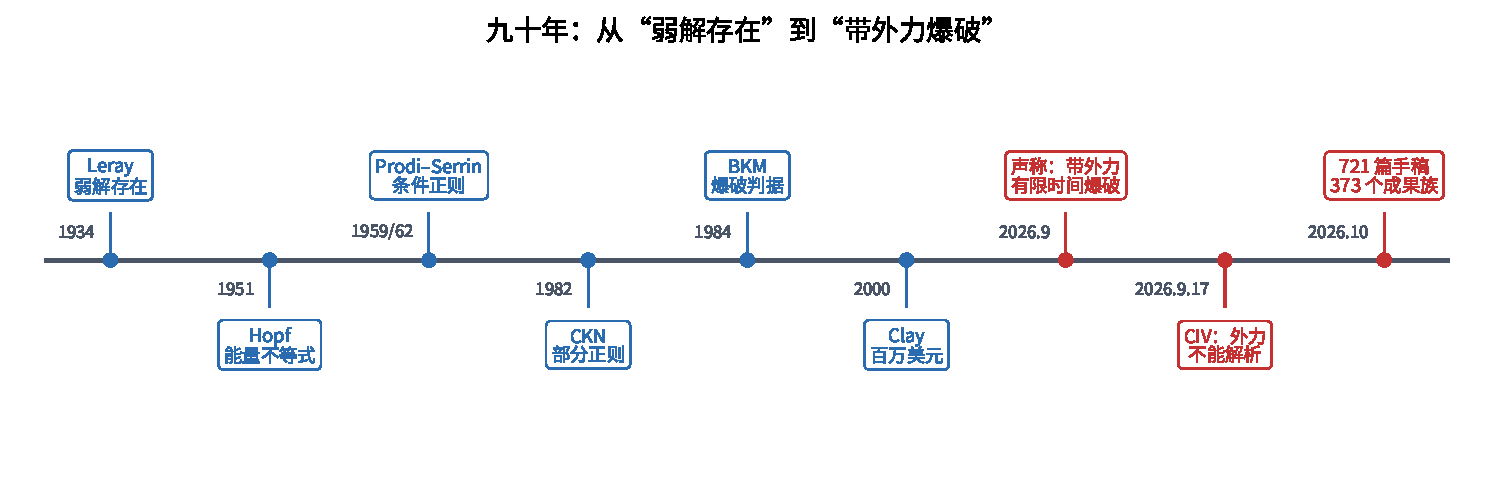
\includegraphics[width=\linewidth]{figs/fig08_timeline.pdf}
\caption{九十年的一条线：从 Leray 的弱解存在性，到 2026 年 9 月的“带外力爆破”声称，
再到一周后 Constantin--Ignatova--Vicol 的“外力不能解析”定理。}
\label{fig:timeline}
\end{figure}

\begin{enumerate}[leftmargin=1.8em]
\item \textbf{Leray--Hopf 弱解（1934/1951）}：对任意 $L^2$ 初值，\emph{总存在}一个
      满足能量不等式的弱解。这是存在性定理，\emph{不}保证唯一，\emph{不}保证光滑。
\item \textbf{Caffarelli--Kohn--Nirenberg 部分正则性（1982）}：三维的奇点集合
      （如果存在）在抛物意义下是一维零测的——也就是说，奇点至多是“一些点/曲线”，
      不能是一整块区域。这条定理对“有”和“没有”两种答案都成立，因此不能定案。
\item \textbf{Prodi--Serrin 条件正则性（1959/1962）}：若解满足
      $u\in L^p_tL^q_x$ 且 $2/p+3/q\le1$（$q>3$），则不会爆破。
      注意 $q=3$ 是临界情形，恰好是开放的。
\item \textbf{Beale--Kato--Majda 判据（1984）}：$\int_0^{T^*}\|\nabla u\|_\infty\,dt<\infty$
      则不爆破。所有现代爆破分析都围绕这个量。
\end{enumerate}

一句话总结：\emph{存在性、部分正则性、条件正则性都有了；缺的是那个无条件的东西。}

\section{转折点：把外力放开会发生什么}\label{sec:prescription}

\subsection{一个“太显然以至于被忽略”的定理}

\begin{keybox}[指定力定理（本文论文第 7 节）]
任给一条光滑、无散的速度路径 $v(x,t)$（$0\le t<T$），令 $q$ 解
$-\Delta q=\operatorname{div}((v\cdot\nabla)v)$，再令
\[
f=\partial_tv+(v\cdot\nabla)v-\nu\Delta v+\nabla q .
\]
那么 $(v,q,f)$ 就是纳维–斯托克斯方程的\emph{精确解}，外力就是这个 $f$。
\end{keybox}

证明只有一行：把 $f$ 代回方程，左右两边相同，且 $\operatorname{div}f=0$ 由 $q$ 的方程保证。

这条定理的哲学含义很重：\textbf{一旦外力完全自由，方程对“路径”没有任何约束。}
你可以让流体做任何事——绕圈、跳舞、在指定时刻爆破——只要相应地设计外力。
换句话说，选项 (C) 不是“解方程”，而是“选路径 + 付账”。

\begin{figure}[htbp]
\centering
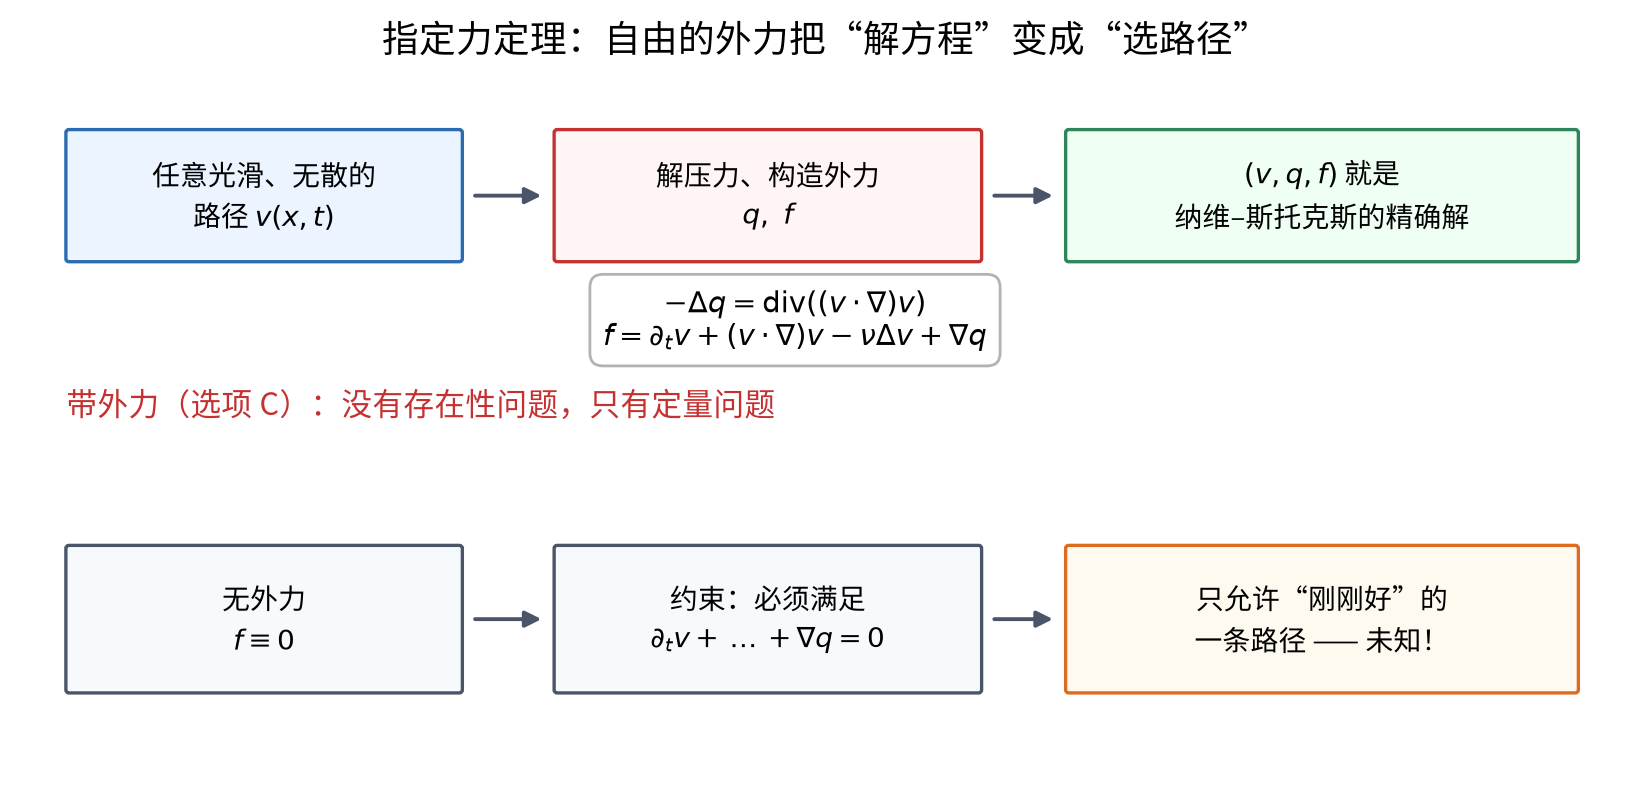
\includegraphics[width=\linewidth]{figs/fig05_prescription.png}
\caption{上：带外力时，任意光滑无散路径都是某个外力的解（指定力定理）。
下：无外力时，路径必须满足一个非线性约束——只允许“刚刚好”的那一条，而我们对它一无所知。}
\label{fig:prescription}
\end{figure}

\subsection{所以“带外力爆破”是容易的}

取一个自相似的路径
\[
v(x,t)=\lambda(t)\,U(\lambda(t)x),\qquad
\lambda(t)=\bigl(2a(T-t)\bigr)^{-1/2},
\]
其中 $U$ 是任意一个光滑、紧支撑、无散的非零场。那么当 $t\uparrow T$ 时
$\lambda\to\infty$，
\[
\|v(t)\|_{\dot H^s}=\lambda^{s-1/2}\|U\|_{\dot H^s}\to\infty\quad(s>1/2),
\qquad
\|v(t)\|_\infty=\lambda\|U\|_\infty\to\infty .
\]
也就是说，\textbf{在任意预先指定的时刻 $T$，任意高的 Sobolev 范数都可以爆破}——
代价是外力按 $\lambda^3$ 增长（图~\ref{fig:manufactured}）。

\begin{figure}[htbp]
\centering
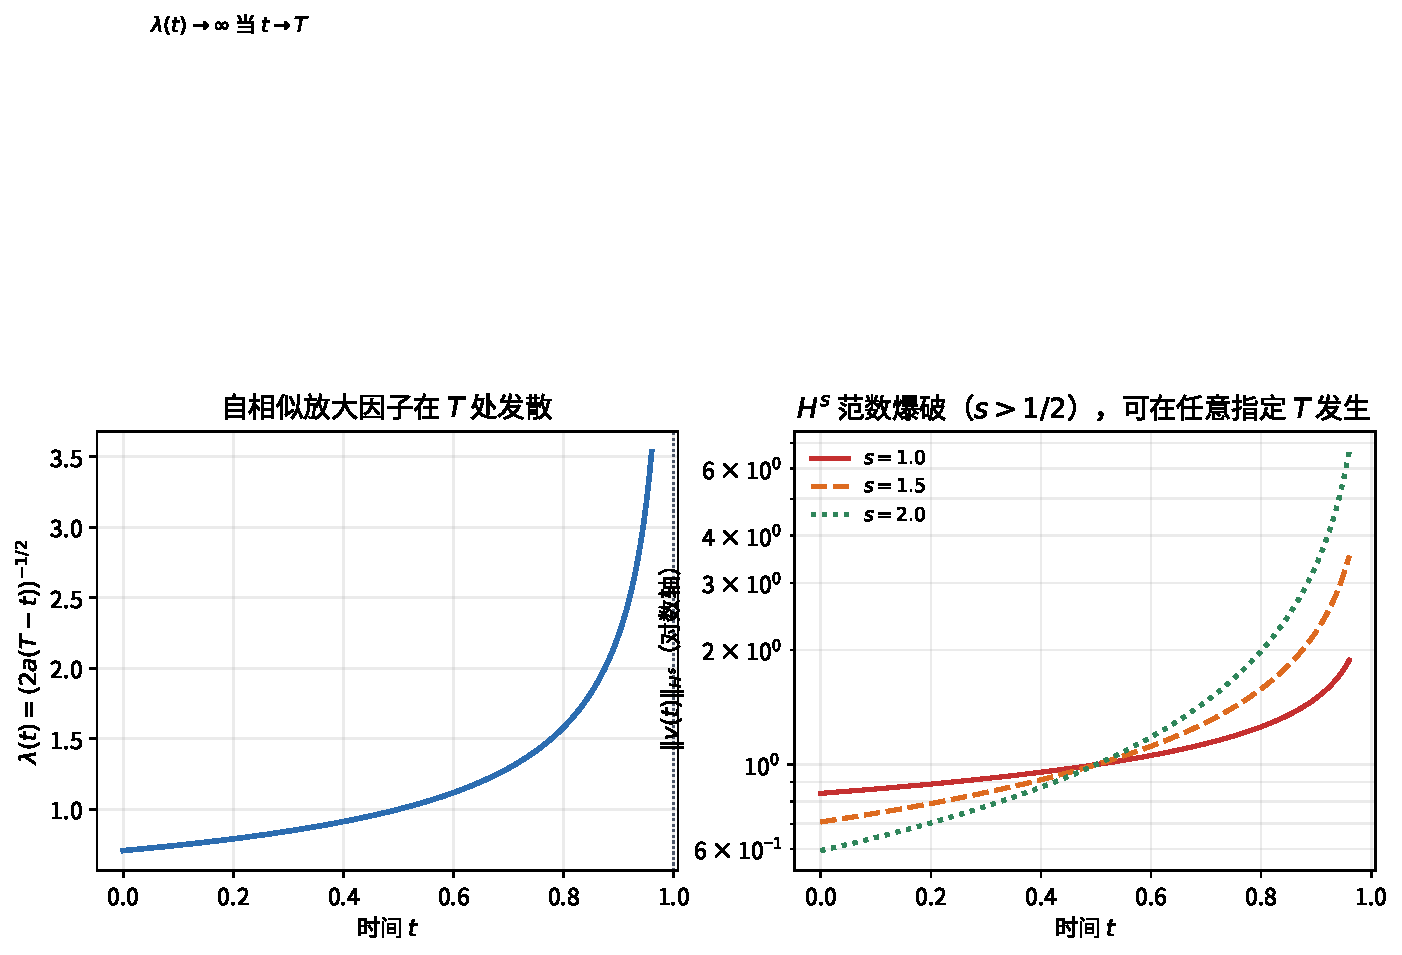
\includegraphics[width=\linewidth]{figs/fig06_manufactured.pdf}
\caption{人造爆破。左：放大因子在 $T$ 处发散。右：$H^s$ 范数（$s>1/2$）随之爆破。
这一切都能在任意指定的 $T$ 发生——但外力也一起爆破。}
\label{fig:manufactured}
\end{figure}

\section{代价定律：外力必须按 $(T-t)^{-3/2}$ 发散}\label{sec:price}

上一节的“人造爆破”看起来像作弊。它当然是，但作弊也有价目表——而且这个价目表是
\emph{被方程本身逼出来的}，不是构造的技巧。

\begin{keybox}[代价定律（本文论文第 8 节）]
设 $(u,p,f)$ 是三维纳维–斯托克斯方程在 $0<t<T$ 上的精确自相似解：
\[
u(x,t)=\lambda(t)U(\lambda(t)x),\qquad
p(x,t)=\lambda(t)^2P(\lambda(t)x),\qquad
\lambda(t)=\bigl(2a(T-t)\bigr)^{-1/2}.
\]
那么外力必然具有形式
\[
f(x,t)=\lambda(t)^3F(\lambda(t)x),\qquad
F=a\bigl(U+y\cdot\nabla U\bigr)+(U\cdot\nabla)U-\nu\Delta U+\nabla P .
\]
于是\emph{精确地}
\[
\|f(t)\|_\infty=(2a)^{-3/2}\|F\|_\infty\,(T-t)^{-3/2}.
\]
\end{keybox}

推导只有三行：$\dot\lambda=a\lambda^3$、
$\partial_tu=a\lambda^3(U+y\cdot\nabla U)$、$(u\cdot\nabla)u=\lambda^3(U\cdot\nabla)U$、
$\Delta u=\lambda^3\Delta U$、$\nabla p=\lambda^3\nabla P$，加起来就是 $\lambda^3F(y)$。

\begin{figure}[htbp]
\centering
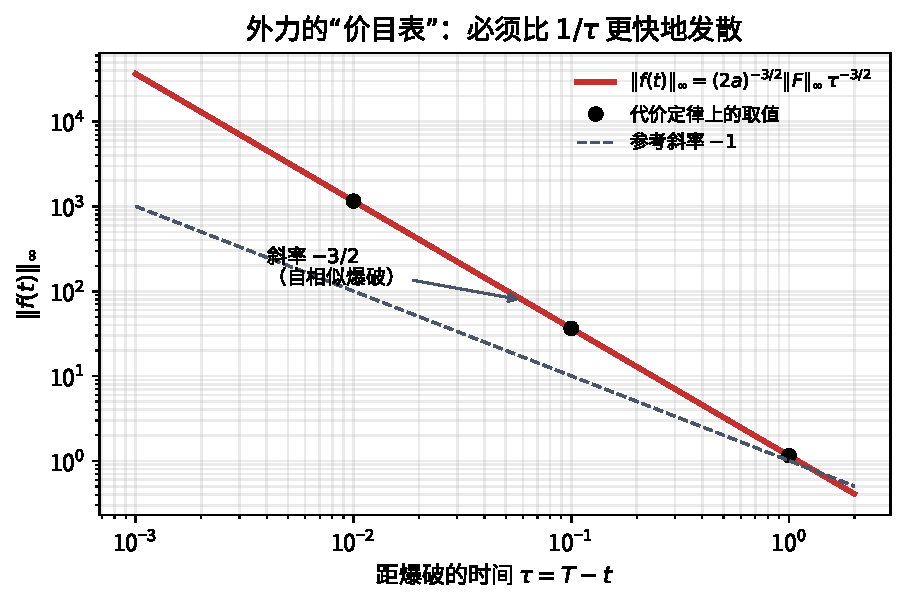
\includegraphics[width=0.76\linewidth]{figs/fig07_price.pdf}
\caption{代价定律的“价目表”（双对数坐标）。红线斜率是 $-3/2$，比 $1/\tau$（灰虚线）
更陡。意思是：越接近爆破时刻，外力必须发散得越快。}
\label{fig:price}
\end{figure}

\subsection{两个直接推论}

\begin{warnbox}[推论 1：有界外力不可能支撑精确自相似爆破]
若 $\sup_{t<T}\|f(t)\|_\infty<\infty$，则 $F\equiv0$，从而 $f\equiv0$。
换句话说：\emph{只要外力在爆破时刻还有界，这种自相似爆破就根本不存在。}
\end{warnbox}

物理翻译：想在一个点上把能量越聚越密，就必须在那一瞬间往那个点注入越来越强的力；
力一旦有界，能量就会被粘性耗散掉，聚不起来。

\begin{warnbox}[推论 2：外力必须“坏”到某种程度]
2026 年 9 月 17 日，Constantin--Ignatova--Vicol 证明：在那个人造爆破的结构假设下，
如果外力在空间变量上是\emph{实解析}的（且对时间一致），解其实是正则的。
由于 $f\equiv0$ 当然解析，在这类构造的结构假设下，这条定理说明：外力不能是解析的，
也不能在奇点附近恒为零。于是“把外力支到奇点之外、让奇点附近变成无外力问题”这条
捷径行不通——除非放弃那两条结构假设，而那就等于换了一个问题。
\end{warnbox}

这就是第 \ref{sec:prescription} 节标题的含义：外力不是装饰，它是答案的一部分。
换一个外力，问题就换了一个。

\section{2026 年到底发生了什么（时间线）}\label{sec:2026}

\begin{enumerate}[leftmargin=1.8em]
\item \textbf{9 月 8 日}：OpenAI 公布一份 166 页手稿和一份 Lean 形式化，声称证明了
      \emph{带光滑外力}的三维纳维–斯托克斯方程存在有限时间爆破。
      对应的是 Clay 官方陈述里允许外力的“选项 (C)”。
\item \textbf{9 月 17 日}：Constantin--Ignatova--Vicol（arXiv:2609.20803）证明：
      在上述结构假设下，若外力在奇点附近解析或恒为零，解其实正则。
      等价地说：那条爆破路线\emph{无法}推广到无外力情形。
      10 月 18 日，Ingimarson--Kukavica--Xu 把“解析”弱化为“外力旋度的旋转不变性”。
\item \textbf{10 月 6 日}：OpenAI 一次性公开 722 篇手稿，归为 372 个“成果族”
      （不是 722 个定理；一个成果族可能包含主结果、伴随论证、替代证明）。
      次日撤回 3 篇（一处符号错误 + 两篇依赖它的论文），修订 14 篇；
      10 月 26 日又加 2 篇。官方仓库现在是 \textbf{721 篇 / 373 族}，
      其中约 42\% 的“头条结果”有 Lean 形式化。
\item \textbf{10 月 6 日}：Bastounis--Circelli--Hansen（arXiv:2610.08144）指出，
      该工作的 Lean 形式化与其自然语言证明\emph{并不对应}；
      并证明“语义忠实的自动形式化”难度高于停机问题。
\item \textbf{官方状态}：Clay 数学研究所仍把该问题列为 \textbf{active}（开放），
      评审“刻意不赶时间”（deliberately unhurried），100 万美元未颁发。
      另有 8000 余名研究者联署批评发布方式，以及一位 NYU 数学家的优先权争议。
\end{enumerate}

注意两件事：\emph{(i)} 9 月那篇爆破论文并不在 10 月的 721 篇合集里
（合集里与纳维–斯托克斯相关的只有“受迫流中的通用计算”那一族）；
\emph{(ii)} “700 多道题”是手稿数，不是“700 多个被解决的问题”。

\subsection{“Lean 验证过”能说明什么}

Lean 是一个证明助手：只要把证明翻译成它的形式语言，机器就能逐步检查。
问题在于\textbf{翻译这一步本身}。图~\ref{fig:lean} 是这条“证据链”：
手稿 $\to$ 同行评审 $\to$ Lean 形式化 $\to$ Clay 评审 $\to$ 奖金。
红色虚线表示：翻译可能不忠实，而判断“是否忠实”这件事，被证明比停机问题还难。
所以“Lean 检查通过”只能说明“某个形式命题有证明”，不能说明“论文里那个命题有证明”。

\begin{figure}[htbp]
\centering
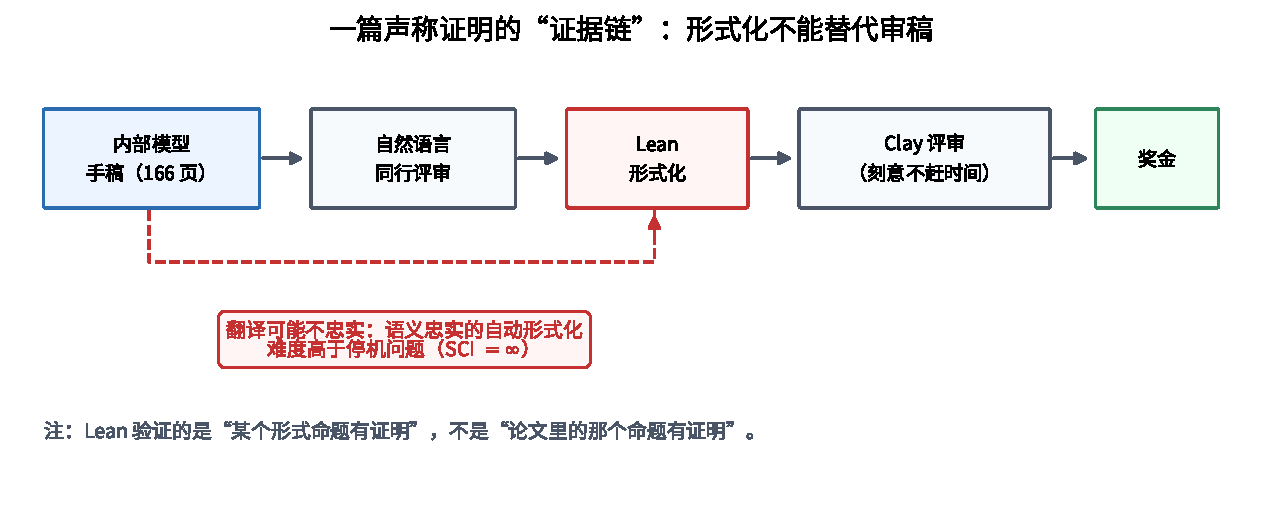
\includegraphics[width=\linewidth]{figs/fig11_lean.pdf}
\caption{一篇声称证明的“证据链”。形式化是强有力的辅助，但它替代不了自然语言的审稿，
因为“忠实翻译”本身不可算法化。}
\label{fig:lean}
\end{figure}

\section{放回千禧七题的框架里}

图~\ref{fig:clay} 是七道题的现状。七道题里只有庞加莱猜想落地（Perelman，2002--03，
还拒领奖金）；其余六道开放。纳维–斯托克斯这一行的橙色标注，是本讲义想强调的：
2026 年的事件让这一行\emph{更热闹}，但没有让它变成绿色。

\begin{figure}[htbp]
\centering
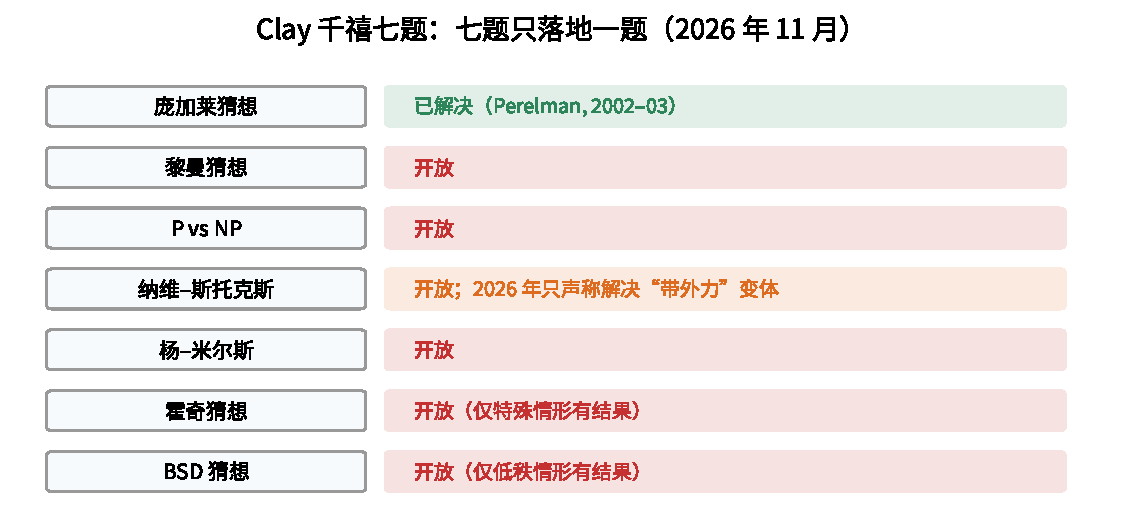
\includegraphics[width=0.92\linewidth]{figs/fig10_clay.pdf}
\caption{Clay 千禧七题现状（2026 年 11 月）。}
\label{fig:clay}
\end{figure}

\section{我们怎么确认自己没有算错}\label{sec:num}

讲义里所有“精确”的公式（$\lambda^3$、$(T-t)^{-3/2}$、$\operatorname{div}f=0$、
二维输运项积分为零）都在配套论文的附录里做了数值核验。
图~\ref{fig:verify} 是误差的条形图：四条绿/蓝条是代数恒等式（误差 $10^{-10}$ 以下，
达到双精度极限），橙条是有限差分带来的截断误差（$10^{-5.6}$，与 $h^2$ 一致）。

\begin{figure}[htbp]
\centering
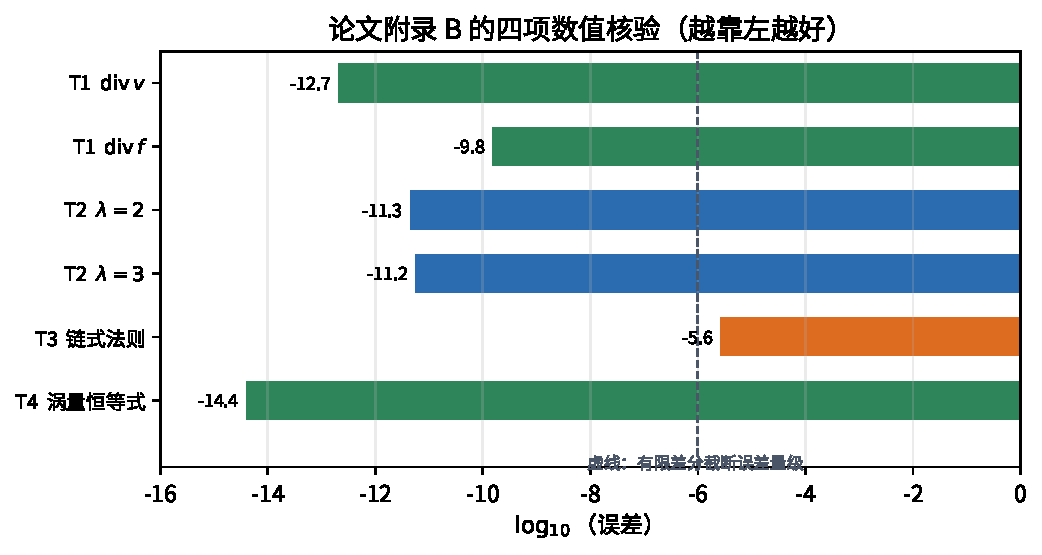
\includegraphics[width=0.86\linewidth]{figs/fig09_verification.pdf}
\caption{四项数值核验的误差（$\log_{10}$，越靠左越好）。
T1 检验压力方程的符号（$\operatorname{div}f=0$ 只在符号正确时成立）；
T2 检验 $\lambda^3$ 指数；T3 检验链式法则与代价定律；T4 检验二维涡量的输运项确实为零。}
\label{fig:verify}
\end{figure}

\begin{keybox}[诚实的边界]
数值核验能确认“代数没写错”，\emph{不能}替代证明。
我们核验的是恒等式，不是“三维永远不爆破”这种全称命题。
\end{keybox}

\section{如何读一条“AI 证明了某某猜想”的新闻}\label{sec:checklist}

下面七个问题，是这次事件里真正决定结论的那七个。建议以后看到类似新闻时逐条对照。

\begin{enumerate}[label=\textbf{Q\arabic*.},leftmargin=2.2em]
\item \textbf{问的是哪个版本？} 有外力还是无外力？$\mathbb{R}^3$ 还是环面？
      衰减还是周期？这三组选择互不等价。
\item \textbf{外力的函数类是什么？} 只要求“在 $[0,T)$ 上光滑”，还是“在 $[0,T]$ 上光滑
      且各阶导数有界”？前者允许 $(T-t)^{-3/2}$ 型发散，后者不允许。
\item \textbf{允许外力在爆破时刻发散吗？} 若允许，速率是多少？是否与代价定律相容？
\item \textbf{用了哪些结构假设？} 轴对称、解析性、Type I/II 界……
      每一条都必须要么从初值推出，要么明写成假设。
\item \textbf{常数对 $t$ 一致吗？} 一个随 $t\uparrow T$ 变坏的界，不能用来做延拓。
\item \textbf{形式化忠实吗？} “Lean 检查通过”$\ne$“论文的命题被证明”。
\item \textbf{计算可复现吗？} 代码、输入、容差是否公开？
\end{enumerate}

把这七条套到 2026 年 9 月那次声称上：
Q1 答“带外力”；Q2 答“$[0,T)$ 上光滑”；Q3 答“必须按 $(T-t)^{-3/2}$ 发散”；
Q4 答“轴对称 + Type II 界”；Q6 答“已有工作指出不忠实”；Q7 答“部分公开”。
于是结论很清楚：\emph{它是一次真实的技术推进，但不是千禧问题的解答。}

\section{结语：三条给普通读者的“抓手”}

\begin{enumerate}[leftmargin=1.8em]
\item \textbf{“存在解”和“解不爆破”是两件事。} Leray 在 1934 年就证了前者；
      后者至今未知。新闻里说“方程有解”，往往只是前者。
\item \textbf{二维和三维的差别只有一项，但这一项足够致命。} 二维涡量只被输运和扩散，
      所以有单调量；三维多了拉伸项，一切单调性消失。
\item \textbf{外力和无外力是两个问题。} 一旦允许自由外力，方程就变成控制问题；
      “能爆破”几乎不要证，真正的问题是“需要多大的外力”。代价定律给出的答案是
      $(T-t)^{-3/2}$，而且在自相似情形下是精确的。
\end{enumerate}

\appendix

\section{配套论文与代码}

\begin{itemize}[leftmargin=1.6em]
\item 论文：\texttt{paper/ns-forced-vs-unforced.pdf}（20 页，英文，含完整证明）
      \begin{itemize}
      \item 定理 4.2：Prodi--Serrin 判据（完整证明）
      \item 定理 4.6：Beale--Kato--Majda 判据（完整证明）
      \item 定理 5.1：二维全局正则性（完整证明）
      \item 定理 7.1：指定力定理（完整证明）
      \item 推论 7.3：人造爆破（完整证明）
      \item 定理 8.1：代价定律 $\|f(t)\|_\infty=(2a)^{-3/2}\|F\|_\infty(T-t)^{-3/2}$（完整证明）
      \item 定理 9.1 + 推论 9.2：CIV 定理及其对 2026 构造的含义
      \end{itemize}
\item 论文源码：\texttt{paper/ns-forced-vs-unforced.tex}（\texttt{tectonic -X compile} 即可）
\item 本讲义的图：\texttt{notes/make\_figs.py}（二维模拟）与
      \texttt{notes/make\_schematics.py}（示意图），输出在 \texttt{notes/figs/}
\item 数值核验：\texttt{paper/verify.py}，输出 \texttt{paper/verify.out}
\end{itemize}

\subsection*{复现二维模拟}

\begin{verbatim}
cd notes
python3 make_figs.py        # 约 1--2 分钟，生成图 2、图 3
python3 make_schematics.py  # 约 20 秒，生成其余示意图
tectonic -X compile notes.tex
\end{verbatim}

模拟参数：$192^2$ 网格、$\nu=2\times10^{-4}$、时间步 $3\times10^{-3}$、
伪谱法（扩散用积分因子精确处理，对流用 RK4），初始为两个同号高斯涡加一个反号涡。
读者可以自行改参数复现图中 $t=20$ 时刻的细丝结构。

\section*{延伸阅读}
\addcontentsline{toc}{section}{延伸阅读}
\begin{itemize}[leftmargin=1.6em]
\item C.~L. Fefferman, \emph{Existence and smoothness of the Navier--Stokes equation},
      Clay Mathematics Institute, 2000.（官方问题陈述）
\item J.~Leray, \emph{Sur le mouvement d'un liquide visqueux emplissant l'espace},
      Acta Math. 63 (1934).（弱解）
\item L.~Caffarelli, R.~Kohn, L.~Nirenberg, \emph{Partial regularity of suitable weak
      solutions of the Navier--Stokes equations}, CPAM 35 (1982).
\item J.~T. Beale, T.~Kato, A.~Majda, \emph{Remarks on the breakdown of smooth solutions
      for the 3-D Euler equations}, Comm. Math. Phys. 94 (1984).
\item P.~Constantin, M.~Ignatova, V.~Vicol, arXiv:2609.20803（2026）.
\item B.~Ingimarson, I.~Kukavica, Q.~Xu, arXiv:2610.25531（2026）.
\item A.~Bastounis, F.~Circelli, A.~C. Hansen, arXiv:2610.08144（2026）.
\end{itemize}

\end{document}




